\chapter{Experimental results}
\label{ch5}

%%%%%%%%%%%%%%%%%%%%%%%%%%%%%%%%%%%%%%%
% IMPORTANT
\singlespacing % THESE THREE
\minitoc % LINES MUST APPEAR IN
\doublespacing % EVERY CHAPTER
% COPY THEM IN ANY NEW CHAPTER
%%%%%%%%%%%%%%%%%%%%%%%%%%%%%%%%%%%%%%%

\section{Data set}


The dataset used in the following experiments is comprised of the top 5 most traded companies in volume according to NASDAQ screener in each sector as per 19\textsuperscript{th} August 2023, listed since 2016 from Jan 1st 2017 until Jan 1\textsuperscript{st} 2022. The resulting companies can be found in Tables \ref{tab:NASDAQ_1} and \ref{tab:NASDAQ_2}  on Appendix \ref{sec::AppendixNasdaqScreener} using the script in Listing \ref{lst:dataGenScript}. The data corresponding to 2017 and 2018 will be used to pre-load the \ac{MPC} with an initial set of data to make predictions with, 2019 will be used as training data, 2020 as validation data and finally 2021 will be used for backtesting.

Both the \href{https://github.com/brunocastroibarburu94/dissertation_msc_2023/blob/main/dissertationFigures/data/cache/Mark1/2023_08_19_16_9_49_915.parq.snappy}{Yahoo Finance ticker data}\footnote{\url{https://github.com/brunocastroibarburu94/dissertation_msc_2023/blob/main/dissertationFigures/data/cache/Mark1/2023_08_19_16_9_49_915.parq.snappy}} and  \href{https://github.com/brunocastroibarburu94/dissertation_msc_2023/blob/main/dissertationFigures/data/cache/NASDAQscreener_Mark1/2023_08_19_17_16_37_731.parq.snappy}{NASDAQ screener data}\footnote{\url{https://github.com/brunocastroibarburu94/dissertation_msc_2023/blob/main/dissertationFigures/data/cache/NASDAQscreener_Mark1/2023_08_19_17_16_37_731.parq.snappy}} is available online on GitHub and are stored in parquet file format whilst compressed with the snappy algorithm.

\clearpage

\begin{lstlisting}[language=Julia,escapeinside={(*}{*)},label={lst:dataGenScript},caption={Data generation script},captionpos=b]
using DataFrames: groupby, combine
bundle_id="Mark1"
cache_dir = joinpath(@__DIR__, "data", "cache")
###    Pick the 5 most traded companies per sector
using AirBorne.ETL.NASDAQ: screener
using AirBorne.Utils: get_latest_N
tickers_df = screener()
filtered_df =tickers_df[[   x!="" ? parse(Int64, x)<2016 : false for x in tickers_df.ipoyear],["symbol","marketCap","sector","volume"]]
filtered_df[!,"volume"]=parse.(Int64,filtered_df[!,"volume"])
filtered_df[!,"marketCap"]=parse.(Float64,filtered_df[!,"marketCap"])
grouped_df = groupby(filtered_df,"sector")
f(sdf)= get_latest_N(sdf,:volume,5;rev=true)
result = combine(grouped_df,f)
store_bundle(tickers_df; bundle_id="NASDAQscreener_"*bundle_id, archive=true, cache_dir=cache_dir)
###    Extract interday date from Yahoo Finance   
using AirBorne.ETL.Cache: store_bundle
# To generate the "demo" data use:
using AirBorne.ETL.YFinance: get_interday_data
using AirBorne.ETL.Cache: store_bundle
using Dates: DateTime, datetime2unix
from = DateTime("2017-01-01"); to = DateTime("2022-01-01")
u_from = string(round(Int, datetime2unix(from)));
u_to = string(round(Int, datetime2unix(to)))
data = get_interday_data(result.symbol, u_from, u_to)
store_bundle(data; bundle_id=bundle_id, archive=true, cache_dir=cache_dir)
@info "Done!"

\end{lstlisting}

\section{Forecasting} \label{sec:ch5_forecast}
This section evaluates the forecasting algorithms to be used by the \ac{MPC} method, the complete development environment to be able to reproduce the results in this Chapter is also available in \href{https://github.com/brunocastroibarburu94/dissertation_msc_2023}{Github}\footnote{\url{https://github.com/brunocastroibarburu94/dissertation_msc_2023}} with this particular experiment being carried out in the file \href{https://github.com/brunocastroibarburu94/dissertation_msc_2023/blob/main/dissertationFigures/Experiment_1.ipynb}{Experiment\_1}\footnote{\url{https://github.com/brunocastroibarburu94/dissertation_msc_2023/blob/main/dissertationFigures/Experiment_1.ipynb}}.


On this experiment each forecasting method for the MPC, being \textbf{Last Value}, \textbf{Linear Regression}, \textbf{\ac{HMM}} and \textbf{Behavioural} will have their parameters tuned in order to minimize the forecasting error between the expected return and the actual returns obtained, these set of parameters will be referred as ``forecasting optimal parameters"".

In the next section (Section \ref{sec:ch5_backtest}) a similar parameter tuning will be produced to optimize overall the returns of the Mean Variance MPC and a comparison with the parameter, and be referred as ``profit optimal paramters".  

\subsubsection{Parameter tuning: Minimization criteria and error functions}

The set of parameters for each method is achieved through the minimization of the \ac{MAE} (\ref{eq::MAE}) of the expected return forecast with respect to the actual returns

\begin{equation}\label{eq::MAE}
    MAE = \frac{1}{A D N} \sum_{i,j,k=1,1,1}^{A,D,N} |r(i,j,k) - \hat{r}(i,j,k)| = \frac{|r(:,:,:) - \hat{r}(:,:,:)|_1}{A D N} 
\end{equation}

Where $A$ is the number of assets considered, $D$ is the number of days forecasted into the future on each forecast execution, $N$ is the total number of forecasts, $\hat{r}(i,j,k)$ is the expected return forecast of forecast $k$ and asset $i$ on the day $j$ into the future and $r(i,j,k)$ is its corresponding actual value. The scale factor $(ADN)^{-1}$ is introduced to reflect this error in terms of the average deviation between $\hat{r}(i,j,k)$ and $r(i,j,k)$. Lastly $|\cdot|_1$ is the norm 1 and the index ``$:$" represents all the entries of a vector in a particular dimension.

To normalize the error with respect to the magnitude of the target the \ac{MAE} is expanded to consider the relative error with the \ac{MRAE}, \ac{MRAE}$_f$ (\ref{eq::MRAEf}) symbolizes the \ac{MRAE} scaling over the returns of a forecast and \ac{MRAE}$_{fd}$ scales over the forecast day combination, since some returns can be 0 scaling over each return is not possible as divison over 0 is not well defined.


\begin{equation}\label{eq::MRAEf}
    \text{MRAE}_f = \frac{1}{N}\sum_{k=1}^N \left( \frac{|r(:,:,k) - \hat{r} (:,:,k)|_1}{|r(:,:,k)|_1 } \frac{1}{A D} \right) 
\end{equation}

\begin{equation}\label{eq::MRAEfd}
    \text{MRAE}_{fd} = \frac{1}{D N}\sum_{j,k=1}^{D,N} \left( \frac{|r(:,j,k) - \hat{r} (:,j,k)|_1}{|r(:,j,k)|_1 } \frac{1}{A} \right) 
\end{equation}


The choice for sum of absolute values is due to its fast computation time and suitability as is by definition the L1-norm in euclidean space. On the next sections the data of 2017 and 2018 is used to preload with past data the algorithms, each forecasting algorithm is tuned by simulating and evaluating the accuracy of the forecast through a set of days in 2019 (training) and 2020  (validation). 

\subsubsection{Parameter tuning: ``Last Value" optimal forecasting parameters}
Figure \ref{fig:ch5_LV_forecast_optimization} shows the effect of changing the past horizon parameter $w_{s\mu}$ of the Last Value algorithm. By increasing the amount of data samples on the training set we see that the both in the training a validation set the profile of the curve remains similar with improved precision by using 20 to 30 days of information, and when using more than 60 samples of data it can be seen incremental gains by keep increasing it. 

\begin{figure}[ht!]
    \centering
    \begin{subfigure}[b]{.7\linewidth}
        \includesvg[width=\linewidth]{imgs/ch5/E1_01_LV_Optimization_20_days_MRAEf.svg}
        \caption{20 days}\label{fig:mouse}
    \end{subfigure}
    
    \begin{subfigure}[b]{.495\linewidth}
         \includesvg[width=\linewidth]{imgs/ch5/E1_01_LV_Optimization_30_days_MRAEf.svg}
        \caption{30 days}\label{fig:gull}
    \end{subfigure}
    \begin{subfigure}[b]{.495\linewidth}
         \includesvg[width=\linewidth]{imgs/ch5/E1_01_LV_Optimization_60_days_MRAEf.svg}
        \caption{60 days}\label{fig:tiger}
    \end{subfigure}
    
    \caption{MRAEf of ``Last Value" forecast against past horizon with simulations over the first 20 (a), 30 (b) and 60 (c) business days of the year.}
    \label{fig:ch5_LV_forecast_optimization}
\end{figure}


Therefore it is concluded that using a past horizon window of at least 20 to 30 business days can provide information that improves the Last Value forecast algorithm.


Using DirectSearch\cite{DirectSearch.jl} the optimal parameters are 58 past data samples with \ac{MRAE}f of 0.9917.

\subsubsection{Parameter tuning: ``Linear Regression" optimal forecasting parameters}
The linear regression has 2 parameters to estimate the expected returns, first the ``expected return window size" and the ``past horizon". Due to the increase in problem dimensionality the optimal forecast parameters are estimated over a window of 20 days in 2019 and validated through 2020.

\begin{figure}[ht!]
    \centering
    \begin{subfigure}[b]{.495\linewidth}
         \includesvg[width=\linewidth]{imgs/ch5/E1_01_LR_Optimization_expectedReturnWindowSize_1_20_days_MRAEf}
        \caption{$w_{\mu{}s}=1$}
    \end{subfigure}
    \begin{subfigure}[b]{.495\linewidth}
         \includesvg[width=\linewidth]{imgs/ch5/E1_01_LR_Optimization_expectedReturnWindowSize_5_20_days_MRAEf.svg}
        \caption{$w_{\mu{}s}=5$}
    \end{subfigure}
    
    \begin{subfigure}[b]{.495\linewidth}
         \includesvg[width=\linewidth]{imgs/ch5/E1_01_LR_Optimization_expectedReturnWindowSize_10_20_days_MRAEf.svg}
        \caption{$w_{\mu{}s}=10$}
    \end{subfigure}
    \begin{subfigure}[b]{.495\linewidth}
         \includesvg[width=\linewidth]{imgs/ch5/E1_01_LR_Optimization_expectedReturnWindowSize_15_20_days_MRAEf.svg}
        \caption{$w_{\mu{}s}=15$}
    \end{subfigure}
    
    \begin{subfigure}[b]{.495\linewidth}
         \includesvg[width=\linewidth]{imgs/ch5/E1_01_LR_Optimization_expectedReturnWindowSize_20_20_days_MRAEf.svg}
        \caption{$w_{\mu{}s}=20$}
    \end{subfigure}
    \begin{subfigure}[b]{.495\linewidth}
         \includesvg[width=\linewidth]{imgs/ch5/E1_01_LR_Optimization_expectedReturnWindowSize_30_20_days_MRAEf.svg}
        \caption{$w_{\mu{}s}=30$}
    \end{subfigure}
    
    \caption{MRAEf of ``Linear Regression",each subfigure corresponds to a different expected return window size ``$w_{\mu{}s}$" setting.}
    \label{fig:ch5_LR_forecast_optimization}
\end{figure}


Figure \ref{fig:ch5_LR_forecast_optimization} shows the behaviour of the \ac{MRAE}f on the Linear Regression forecast under different values of past horizon and expected return window size, each subfigure corresponds to a different expected return window size. 

From the charts it can be observed that consistently using 20 days as the past horizon reduces the error to a magnitude of 0.002, and that any value of $w_{\mu{}s}$ from 10 onwards reduces significantly the error on short past horizons as expected .

Using DirectSearch\cite{DirectSearch.jl} the optimal parameters are 21 past data samples with a expected return window size of 17 days with a \ac{MRAE}f of 0.9777.
% [ Info: Functions set
% [ Info: [1, 2] : 6.771885344475016, 6.23101813225427
% [ Info: [1, 5] : 2.496915155058229, 2.1701012068068986
% [ Info: [1, 10] : 1.6373803941422909, 1.450347257863957
% [ Info: [1, 15] : 1.3652789261278486, 1.2547066888171658
% [ Info: [1, 20] : 1.2020148996397158, 1.1663720149860604
% [ Info: [1, 30] : 1.1005467640362596, 1.0762880418079623
% [ Info: [5, 2] : 1.9163782543340993, 1.7218304417998482
% [ Info: [5, 5] : 1.582510456656229, 1.4425353318500467
% [ Info: [5, 10] : 1.4627363443554295, 1.2931346623386957
% [ Info: [5, 15] : 1.2862970330499948, 1.1919188375710388
% [ Info: [5, 20] : 1.1646787329575412, 1.125985560997463
% [ Info: [5, 30] : 1.0968482008138838, 1.0794856836091828
% [ Info: [10, 2] : 1.3543040359039729, 1.2553885121663406
% [ Info: [10, 5] : 1.2338396116027688, 1.156095363490553
% [ Info: [10, 10] : 1.2039541413125163, 1.1385710740783141
% [ Info: [10, 15] : 1.1565998398917434, 1.112342887704466
% [ Info: [10, 20] : 1.1103418457518328, 1.0798684127855829
% [ Info: [10, 30] : 1.086982319713225, 1.08638530004482
% [ Info: [15, 2] : 1.177222920048255, 1.13711351071236
% [ Info: [15, 5] : 1.0795503686674675, 1.0790764643011592
% [ Info: [15, 10] : 1.07498047971579, 1.063598920228684
% [ Info: [15, 15] : 1.0694144906863678, 1.055752775326467
% [ Info: [15, 20] : 1.06551381960916, 1.0587386112608013
% [ Info: [15, 30] : 1.0646630572414957, 1.0779647874231992
% [ Info: [20, 2] : 1.0792869817840571, 1.1084792187121466
% [ Info: [20, 5] : 1.0456925593451207, 1.0617601709265816
% [ Info: [20, 10] : 1.0440637096264136, 1.0482087694395645
% [ Info: [20, 15] : 1.0428176468580963, 1.049503506650027
% [ Info: [20, 20] : 1.0514006885004037, 1.0645860970688314
% [ Info: [20, 30] : 1.0371027760688256, 1.0643585632405796
% [ Info: [30, 2] : 1.0382543415737289, 1.0616367983157884
% [ Info: [30, 5] : 1.0316789988102353, 1.069799384649522
% [ Info: [30, 10] : 1.03538633727675, 1.060376110352219
% [ Info: [30, 15] : 1.0198560971683028, 1.0432996989242362
% [ Info: [30, 20] : 1.0041737588384678, 1.030527128485835
% [ Info: [30, 30] : 0.9943790603005871, 1.0249398362107487

\subsubsection{Parameter tuning: ``Behavioural" optimal forecasting parameters}
Figure \ref{fig:ch5_BF_forecast_optimization_60} shows the effect of varying the past horizon parameter on the behavioural algorithm for the prediction of the expected returns 7 days into the future over a set of 60 days in 2019, training, and 2020, validation. The overall accuracy of the method does not seem to be affected by introducing additional past data points. 

\begin{figure}[ht!]
    \centering
    \includesvg[width=0.7\linewidth]{imgs/ch5/E1_01_BH_Optimization_60_days_MRAEf.svg}
    \caption{Optimization of behavioural forecasting past horizon parameter.}
    \label{fig:ch5_BF_forecast_optimization_60}
\end{figure}

Using DirectSearch\cite{DirectSearch.jl}, the optimal parameter is estimated to be 4 with a \ac{MRAE}f of 3.3341. However is worth pointing out that this parameter may be just a local minima due to the characteristics of the dataset, and not a true optimal parameter, as following Figure \ref{fig:ch5_BF_forecast_optimization_60} no clear trend in the data is observable.

% [ Info: Functions set: Behavioural(20 day MaxSimIter)
% [ Info: [2] : 0.005597675992029323, 0.0059506531078460335
% [ Info: [5] : 0.015568378138412685, 0.04204245030948035
% [ Info: [10] : 0.2558385245696765, 0.03463112398657034
% [ Info: [15] : 0.007290825233809314, 0.018496722822520517
% [ Info: [20] : 0.0006332719486116302, 0.0004572517418737971
% [ Info: [25] : 0.0006332719486116611, 0.0004572517418738219
% [ Info: [30] : 0.0006332719486116399, 0.0004572517418738346
% [ Info: [35] : 0.0006332719486116731, 0.000457251741873812
% [ Info: [40] : 0.0006332719486116629, 0.00045725174187382826
% [ Info: [45] : 0.0006332719486116737, 0.0004572517418739031
% [ Info: [50] : 0.0006332719486116598, 0.0004572517418745848

% [ Info: Functions set: Behavioural
% [ Info: [ 2] : 0.005594516677291844, 0.015250970869184765
% [ Info: [ 5] : 0.017852960079913303, 0.07378624501761286
% [ Info: [ 10] : 0.011149363778533069, 0.027603033216353153
% [ Info: [ 15] : 0.02975079416339273, 0.04169939016269818
% [ Info: [ 20] : 0.019309924794808836, 0.18505432417249287
% [ Info: [ 25] : 0.03649786054483885, 0.035633313705325693
% [ Info: [ 30] : 0.0004053484249856771, 0.00027784408992802457
% [ Info: [ 35] : 0.0004053484249856967, 0.0002778440899280291
% [ Info: [ 40] : 0.0010702650986366467, 0.0002778440899280341
% [ Info: [ 45] : 0.00040534842498568947, 0.000277844089928035
% [ Info: [ 50] : 0.00040534842498570053, 0.0002778440899281476

% [ Info: Functions set: Behavioural
% [ Info: [ 2] : 0.00906723112551376, 0.0783953848461613
% [ Info: [ 5] : 0.01632464794896272, 0.11358495443839277
% [ Info: [ 10] : 0.020434711570278846, 0.08962561422970608
% [ Info: [ 15] : 0.013841716773875554, 0.040187386371491385
% [ Info: [ 20] : 0.017468641370562223, 0.08986057376634213
% [ Info: [ 25] : 0.031587631727219165, 0.0915045920596121
% [ Info: [ 30] : 0.046035379523875285, 0.014767147278958927
% [ Info: [ 35] : 0.023832434225078563, 0.04212104010024474
% [ Info: [ 40] : 0.03853963401956037, 0.07424579803941493
% [ Info: [ 45] : 0.04871072015083477, 0.07973069908465488
% [ Info: [ 50] : 0.021440005325453138, 0.040678853665730035

\subsubsection{Parameter tuning: ``HMM"}
The hyper parameters of \ac{HMM} are the amount of past events used to estimate the model as well as the number of states used, however given the specifications of \cite{MultiPeriod_PO_mpc} a vast amount of past data needs to be used to tune the models, in the original paper 10 years of data was used with the point of capturing different market regimes, in this case 2 years of data will be used. Moreover the usage of 2 states is suggested in previous research \cite{MultiPeriod_PO_mpc}.

\subsection{Conclusions}


\begin{figure}[ht!]
    \centering
    \includesvg[width=\linewidth]{imgs/ch5/E1_01_methodComparison_wo_BH.svg}
    \caption{MRAEf comparison between the methods (excluding behavioural) against the prediction day into the future over 2020}
    \label{fig:comparisonOnlyMu}
\end{figure}


\begin{figure}[ht!]
    \centering
    \includesvg[width=\linewidth]{imgs/ch5/E1_01_methodComparison.svg}
    \caption{MRAEf comparison between the methods against the prediction day into the future over 2020}
    \label{fig:comparisonOnlyMu2}
\end{figure}
% \begin{figure}[ht!]
%     \centering
%     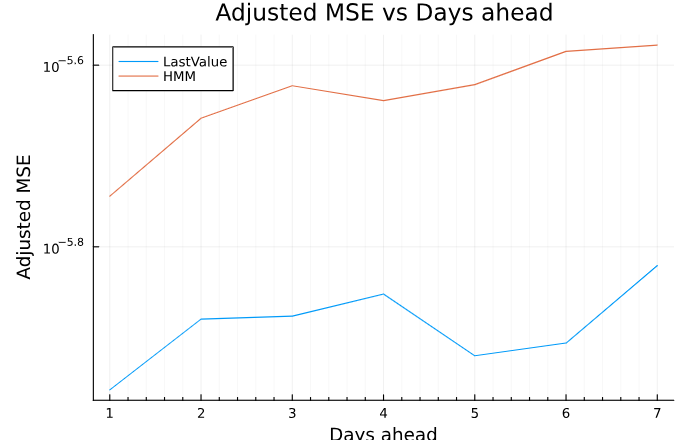
\includegraphics[width=0.7\linewidth]{imgs/ch5/00_raw_comparison_methods.png}
%     \caption{Non tuned variance adjusted comparison between forecasting methods that can produce forecast for the variance }
%     \label{fig:adjustedcomparisonOnlyMu}
% \end{figure}

\clearpage

\section{Backtesting} \label{sec:ch5_backtest}

\subsection{Methodology}

\subsection{Results}
\begin{figure}[ht!]
    \centering
    \includesvg[width=0.7\linewidth]{imgs/ch5/E1_02_BH_Forecast.svg}
    \caption{Portfolio value using Mean-Variance MPC strategy with behavioural forecast.}
    \label{fig:MPC_Behavioural}
\end{figure}

\begin{figure}[ht!]
    \centering
    \includesvg[width=0.7\linewidth]{imgs/ch5/E1_02_LV_Forecast.svg}
    \caption{Portfolio value using Mean-Variance MPC strategy with Last Value forecast.}
    \label{fig:MPC_LV}
\end{figure}

\textbf{Profit optimization parameters:} A second optimization round is performed to compare the result of the forecast error optimization parameters with the optimized profits parameters.

\begin{figure}[ht!]
    \centering
    \includesvg[width=0.7\linewidth]{imgs/ch5/E1_02_BH_Forecast_Optimized.svg}
    \caption{Portfolio value using Mean-Variance MPC strategy with behavioural forecast and profit optimization parameters.}
    \label{fig:MPC_BehaviouralTuned}
\end{figure}

\subsubsection{Benchmarks}


\begin{figure}[ht!]
    \centering
    \includesvg[width=\linewidth]{imgs/ch5/E1_02_best_static_asset_return_all.svg}
    \caption{Returns of all assets.}
    \label{fig:E1_02_best_static_asset_return_all}
\end{figure}

\subsection{Conclusions}

The software for algorithmic trading work, some computational efficiencies can be introduced, particularly for parameter optimization, namely the bottleneck lies on the simulation and lack of gradient descent methods when exploring the parameter space, parallelism can help explore many possibilities simultaneously...